\newpage
\section{Setup for training and testing} % pensare a un titolo
\label{sec:training and testing setup}
Since the goal of this thesis is not to create a new type of generative adversarial network, a pre-existing one have been utilised. The aim was to train the existing network, specifically the ReStyle scheme, discussed in~\ref{section:restyle}, over a variation of the encoder proposed in the pSp framework~(\ref{section:pspFramework}), to generate high-quality face images when conditioned with face sketches. 
%This approach allowed for a more efficient and effective solution as the network had already been pre-trained and had a solid foundation to build upon. 
The dataset used to train the model is the one obtained utilising the techniques explained in~\ref{section:datasetChapter}.
%
\subsection{Training's setup}
%\textbf{Training's setup} \\
The official version of ReStyle published by Alaluf~\cite{alaluf2021restyle} is used as a base model to perform the training.

\noindent The model has been trained on NVIDIA GRID A100D-2-20C GPU, with 11.4 CUDA, and \num{20}GB of memory.

\noindent The training process involves setting up the dataset to be used with ReStyle, therefore the following updates in the \href{https://github.com/yuval-alaluf/restyle-encoder}{ReStyle directory} are needed. The \textit{config/path\_configs.py} has to be update indicating the position where the images, for both training and testing, are saved:
\begin{lstlisting}[language=Python, numbers=none]
    dataset_paths = {
        's_train': 'ffhq/sketch/',
        'f_train': 'ffhq/orig/',
        's_test':  'ffhq/sketch_test/',
        'f_test':  'ffhq/orig_test/'
    }
\end{lstlisting}
The \textit{configs/paths\_config.py} has to be updated, defining the path to the images that have to be used for training and testing. The dataset has to be configured in this way:
\begin{lstlisting}[language=Python, numbers=none]
    DATASETS = {
        'sketch_to_face': {
            'transforms': transforms_config.SketchToImageTransforms,
            'train_source_root': dataset_paths['s_train'],
            'train_target_root': dataset_paths['f_train'],
            'test_source_root':  dataset_paths['s_test'],
            'test_target_root':  dataset_paths['f_test'],
        }
    }
\end{lstlisting}
In the \textit{config/transforms\_configs.py} this code has to be added:
\begin{lstlisting}[language=Python, numbers=none]
    class SketchToImageTransforms(TransformsConfig):
        def __init__(self, opts):
            super(SketchToImageTransforms, self).__init__(opts)
    
        def get_transforms(self):
            transforms_dict = {
                'transform_gt_train': transforms.Compose([
                    transforms.Resize((256, 256)),
                    transforms.ToTensor(),
                    transforms.Normalize([0.5, 0.5, 0.5], [0.5, 0.5, 0.5])]),
                'transform_source':  transforms.Compose([
                    transforms.Resize((256, 256)),
                    transforms.ToTensor()]),
                'transform_test': transforms.Compose([
                    transforms.Resize((256, 256)),
                    transforms.ToTensor(),
                    transforms.Normalize([0.5, 0.5, 0.5], [0.5, 0.5, 0.5])]),
                'transform_inference': transforms.Compose([
                    transforms.Resize((256, 256)),
                    transforms.ToTensor(),
                    transforms.Normalize([0.5, 0.5, 0.5], [0.5, 0.5, 0.5])])
            }
        return transforms_dict
\end{lstlisting}
 Additionally, the \textit{StyleGAN} and \textit{IR-SE50} pre-trained models have to be downloaded and placed in the \textit{pretrained\_models} folder.
 Once all of these steps are performed, the training phase can start using the following command:
 \begin{lstlisting}[language=Python, numbers=none]
    python scripts/train_restyle_psp.py \
    --dataset_type=sketch_to_face \
    --encoder_type=BackboneEncoder \
    --exp_dir=experiment/restyle_psp_s_encode \
    --workers=8 \
    --batch_size=8 \
    --test_batch_size=8 \
    --test_workers=8 \
    --val_interval=5000 \
    --save_interval=10000 \
    --start_from_latent_avg \
    --lpips_lambda=0.8 \
    --l2_lambda=1 \
    --w_norm_lambda=0 \
    --id_lambda=0.1 \
    --input_nc=6 \
    --n_iters_per_batch=5 \
    --output_size=1024 \
    --stylegan_weights=pretrained_models/stylegan2-ffhq-config-f.pt
 \end{lstlisting}
where \textit{dataset\_type} is used to specify the name of the dataset to employ and  \textit{encoder\_type} define the encoder type to apply, that in the case of facial domain is the \textit{BackboneEncoder}. 
The parameter \textit{exp\_dir} indicates the output directory in which the generated images and the weights of the network will be saved. 
\textit{workers} and \textit{test\_workers} represent the number of subprocesses that are activated to speed up the training process by dividing the workload among them. 
The \textit{batch\_size} and \textit{test\_batch\_size} are the number of samples that are passed into the training loop at each iteration. 
The parameter \textit{val\_interval} is used as a validation parameter to evaluate the performance of the model when the global step is a multiple of this parameter. 
\textit{save\_interval} parameter is used to define after how many steps the model has to be saved. To indicate the will to start from an average image, the parameter \textit{start\_from\_latent\_avg} has to be included, and this image is the one showed in Fig.~\ref{fig:Average image}. The parameter \textit{lpips\_lambda}, \textit{l2\_lambda}, \textit{w\_norm\_lambda} and \textit{id\_lambda} are the $\lambda_i$ used to weight differently the various losses defined in~\ref{section:pspFramework}.
To specify the number of iteration for each batch and the output image size, the input parameters to set are \textit{n\_iter\_per\_batch} and \textit{output\_size} respectively. The last parameter is used to specify the path to the directory which contains the weights of the pretrained StyleGAN2 generator.\\
\begin{figure}[htbp]
\centering
  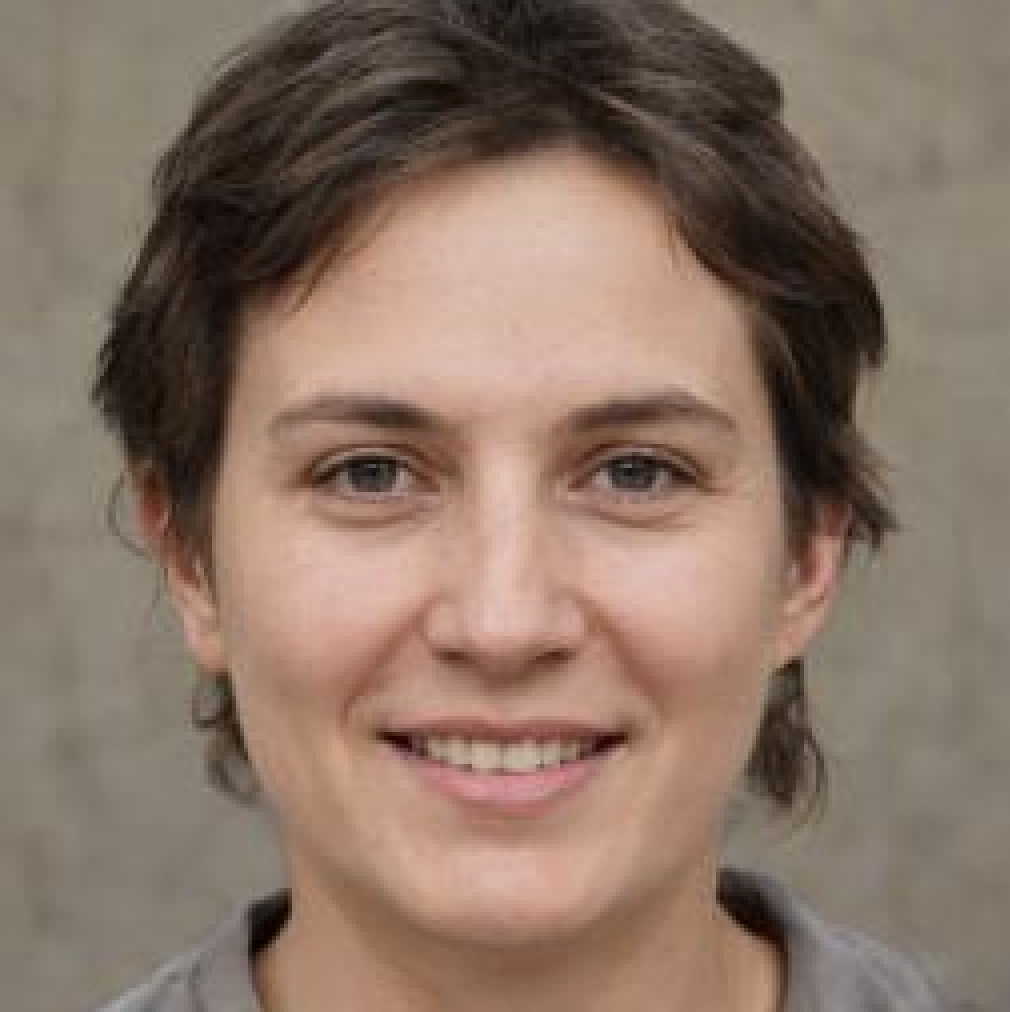
\includegraphics[scale=0.2]{figures/avg_image.png}
  \caption{Average image used}
  \label{fig:Average image}
\end{figure}
%\subsection{Training}
% HO UN PEZZO DI SCRITTE SULLE NOTE NEL CASO VOLESSI AGGIUNGERE L'ADDESTRAMENTO FATTO SUL PRIMO DATASET PERò NON HO I RISULTATI FINALI

\noindent Initially, the first dataset was used to train the network for a duration of three days. However, the results obtained from this training were not up to the expected standards. Subsequently, the second dataset was employed for training the network from scratch for three days. This resulted in a noticeable improvement in the network's performance. Nevertheless, some crucial features were still missing from the output when testing the model. For example, when the sketch presented a person with the beard in the generated image this detail did not appear, and the same happened for details like dimples and wrinkles. To address this, the network was further trained for other three days. Indeed, the model was trained for a total of 70'000 iterations and the end result was a trained generative adversarial network capable of producing realistic face images when conditioned on input sketches.

\noindent In Fig.~\ref{fig:training results} it can be seen the result of the training phase.
\begin{figure}[htbp]
    \centering
    \subfloat[][\emph{Train: 30'000-th iteration}]
    {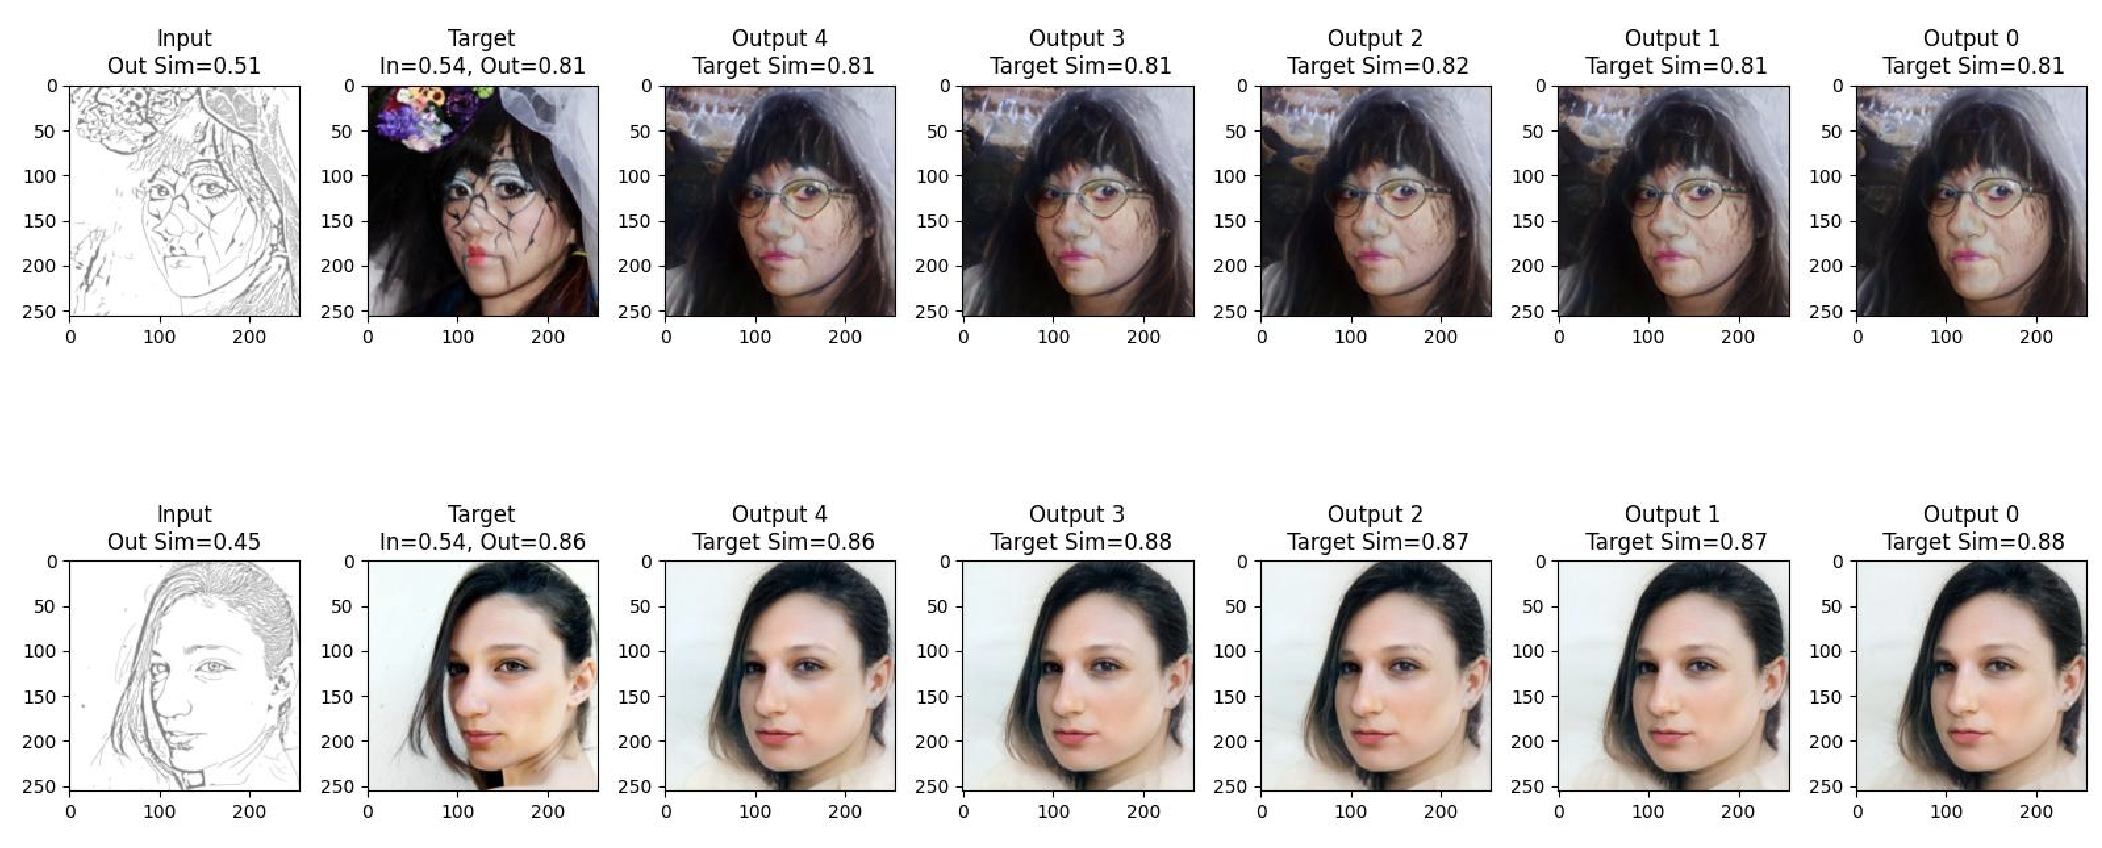
\includegraphics[width=.8\textwidth]{figures/train3000-2db.png}} \quad
    \subfloat[][\emph{Train: 70'000-th iteration}]
    {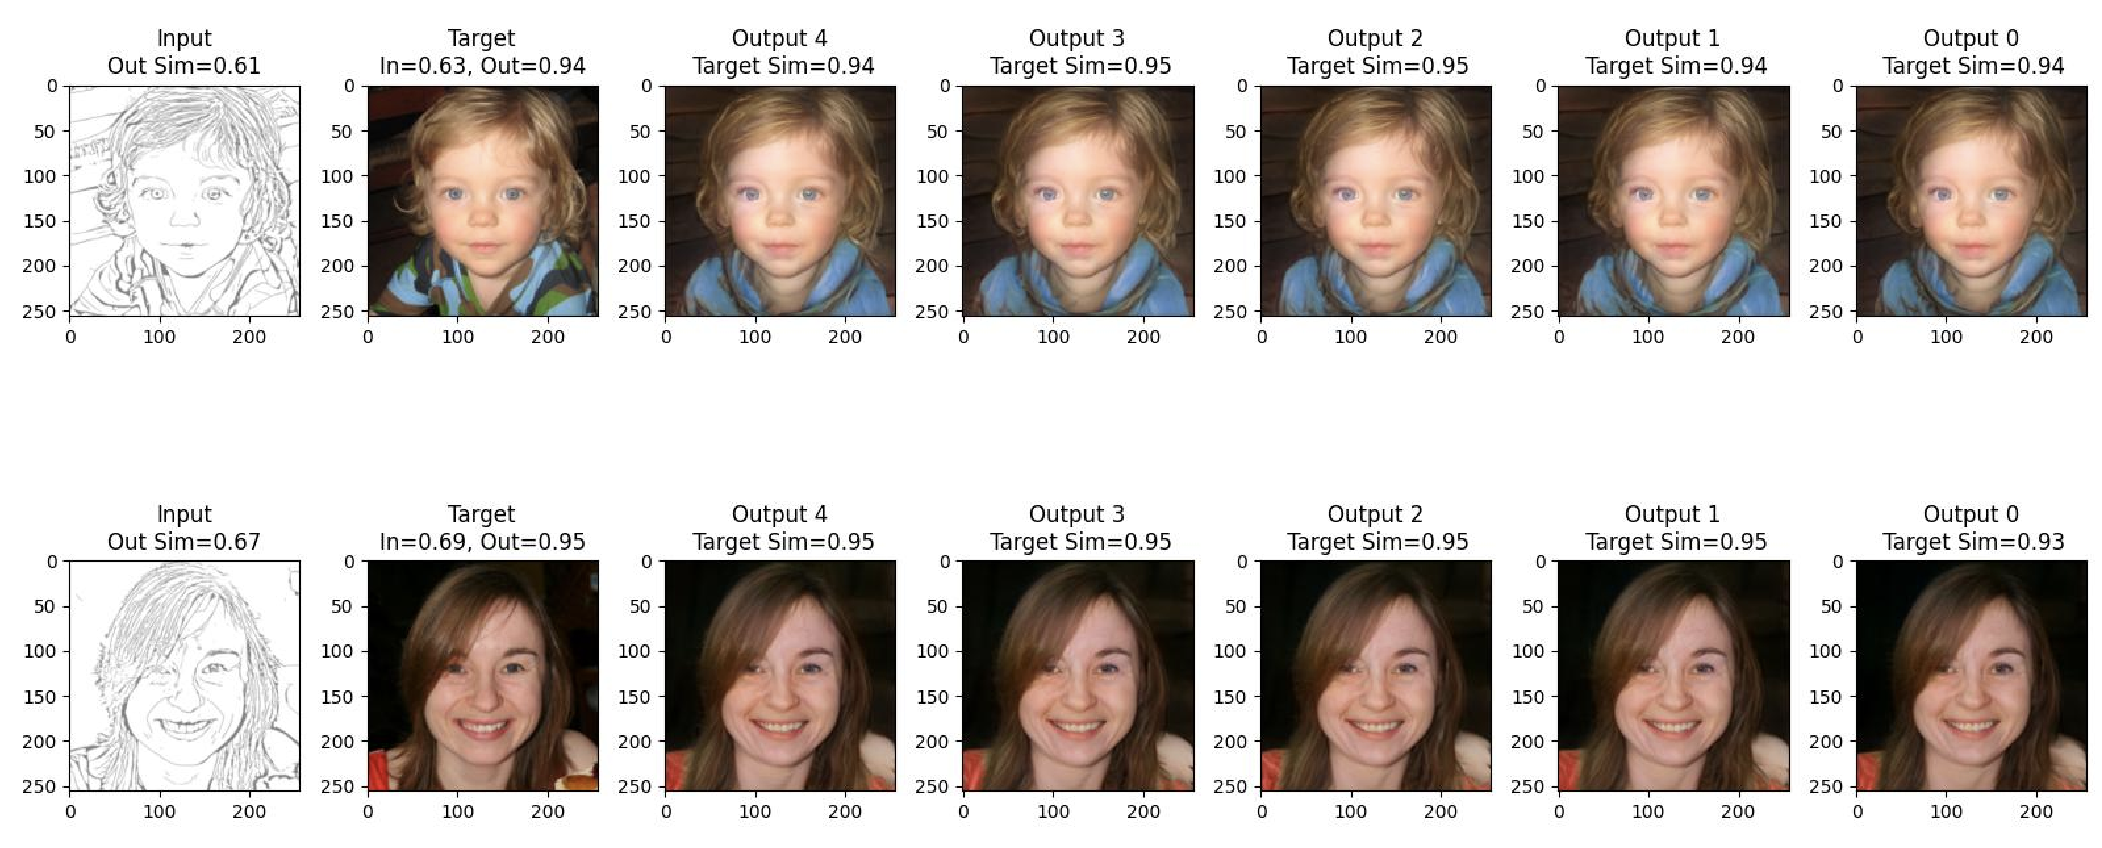
\includegraphics[width=.8\textwidth]{figures/train70000-2DB.png}}\\
    \caption{Training results}
    \label{fig:training results}
\end{figure}
%%%
%
%
\subsection{Testing's setup}
\label{sec:testing setup}
For the purpose of generating synthetic images with the trained model, a graphical user interface has been developed, along with a client-server architecture. All these three are done in Python using the \textit{RPyC} library. This setup enables the model to be tested in a convenient and efficient manner, as the graphical interface provides an easy-to-use interface for inputting data and analysing the results, while the client permits to test the model from the command line inputting existing sketches.
\newline

%\subsubsection{Graphical user interface}
\noindent \textbf{Graphical user interface}

%\label{sec:graphical interface}
\noindent The graphical user interface was done using \textit{Tkinter} library, which allows users to draw on a canvas using a black pen. Additionally, users can use a rubber to delete portions of the sketch, or directly remove the previous inserted lines using the “undo” button, or also clear the canvas, with the “delete” button, and start again from scratch. The rubber and the pen can vary in thickness between 1 (thinner) and 10 (thicker). 
Furthermore, three dashed lines are present, one is vertical in the centre of the interface and the other two are horizontal and placed at eye and chin level. Those lines guide the users in positioning main facial features like the eyes, nose, and mouth. The Fig.~\ref{fig:Graphical interface} shows a sketch drawn on the interface.

\noindent Once the “send” button is pressed, the drawing is sent to the server.
To start the interface, the following command has to be executed.
\begin{lstlisting}[numbers=none]
    python interface.py [-h] [-p PORT] [-a HOST]
    Options:
      -h                this help
      -p PORT           remote server port, default: 18862
      -a HOST           remote server address, default: 140.105.164.237
\end{lstlisting}
\begin{figure}[htbp]
\centering
  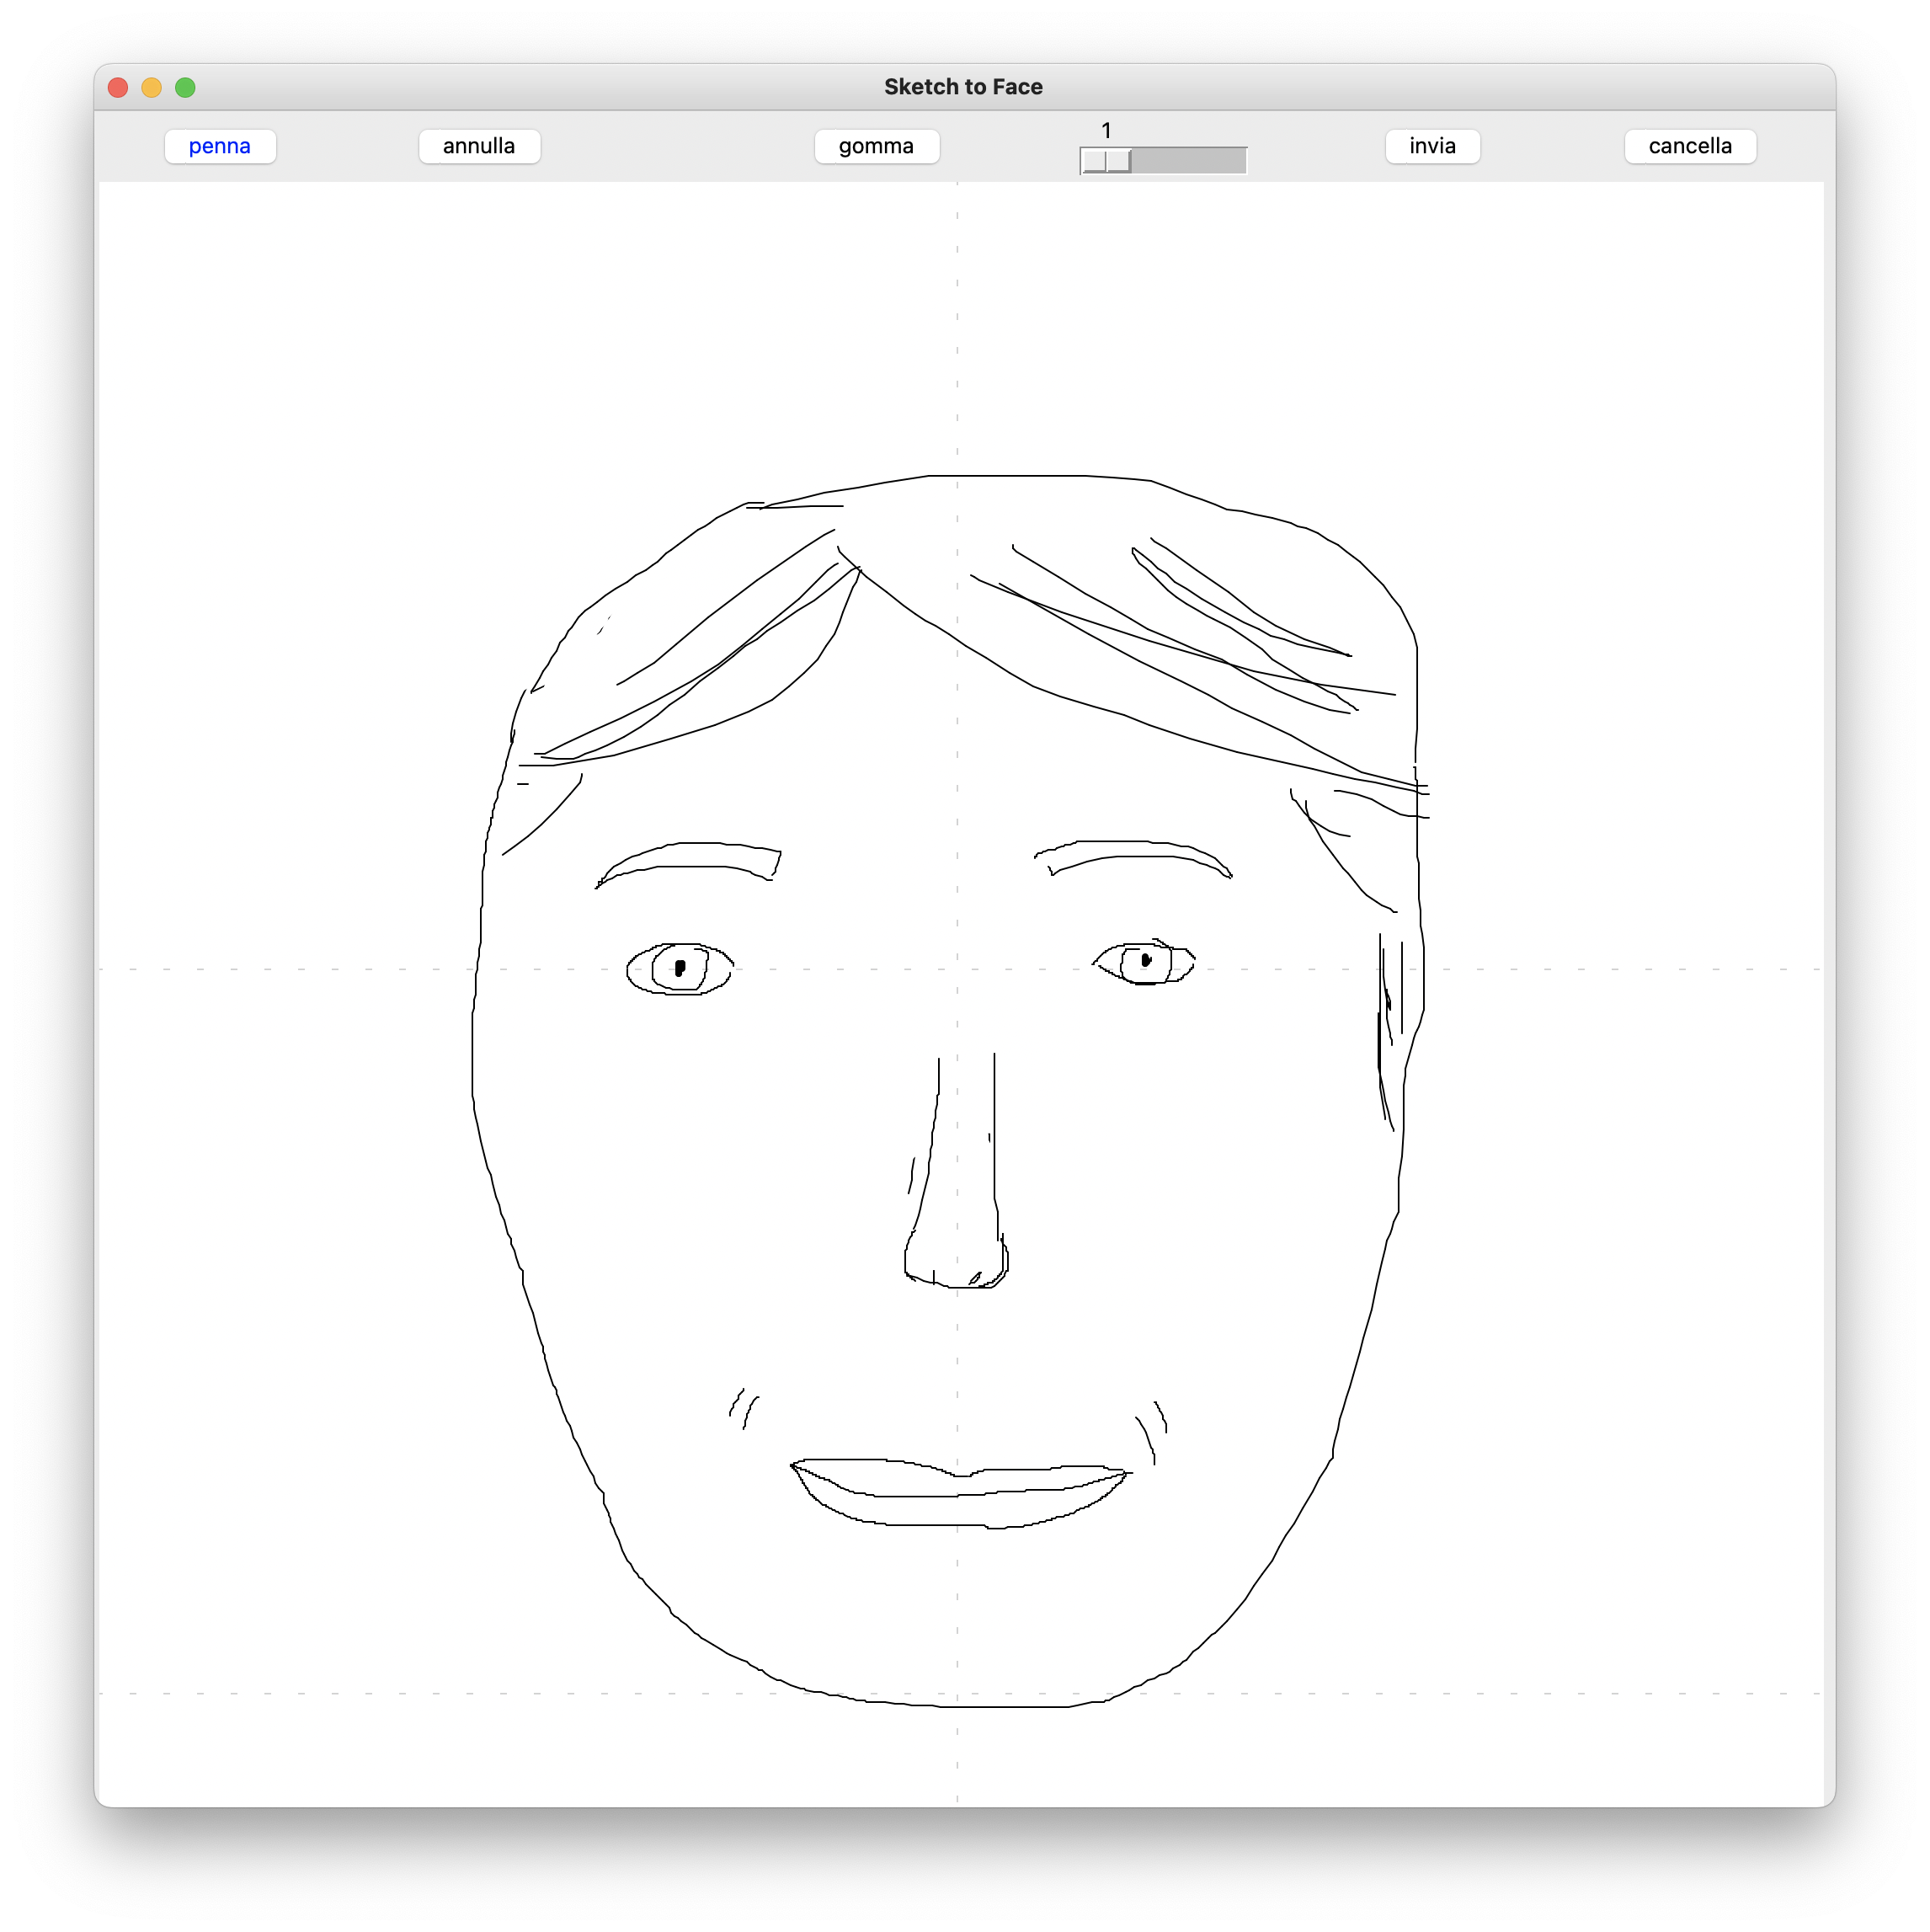
\includegraphics[scale=0.15]{figures/interface.png}
  \caption{Graphical interface}
  \label{fig:Graphical interface}
\end{figure}
\medskip
%\subsubsection{Client architecture}
\textbf{Client architecture}

\noindent An image can also be generated from the command line typing:
\begin{lstlisting}[numbers=none]
    python client_next.py [-h] -i IMAGE [-o OUT] [-p PORT] [-a HOST]
    Options:
      -h                this help
      -i IMAGE          input image
      -o OUT            output file, default: output_results.jpg
      -p PORT           remote server port, default: 18862
      -a HOST           remote server address, default: 140.105.164.237
\end{lstlisting}
The input sketch has to be specified, while there are other parameters that can be set are not mandatory.\\ 
% It opens an image file using the Pillow library and converts it to RGB format. The image is then saved to a buffer and converted to a string. The code then uses the rpyc.connect() method to connect to the server at the specified host name and port. It then calls the exposed\_get\_face method from the root object on the remote server and passes the image string to it. The response from the server is received as a base64-encoded string and is decoded to an image, which is then saved to the specified file.\\
%
%\subsubsection{Server architecture}

\noindent\textbf{Server architecture}

\noindent To be able to generate the image based on the sketches the server has to be up, therefore the following command has to be executed otherwise it will not be possible to generate images.
\begin{lstlisting}[numbers=none]
    python server_next.py [-h] -m MODEL [-t TYPE] [-p PORT]
    Options:
      -h                this help
      -m MODEL          pretrained model
      -t TYPE           type of the mode, either psp or e4e, default: psp
      -p PORT           remote server port, default: 18862
\end{lstlisting}
Once an image is sent to the server, the restyle encoder is applied to generate the output image, which is then sent back as a byte stream and then saved as a PNG image. The server allows also multiple clients since it used the \textit{ThreadedServer} class of \textit{RPyC}.
